% \documentclass[hidelinks,12pt]{article}
\usepackage[left=0.25cm,top=1cm,right=0.25cm,bottom=1cm]{geometry}
%\usepackage[landscape]{geometry}
\textwidth = 20cm
\hoffset = -1cm
\usepackage[utf8]{inputenc}
\usepackage[spanish,es-tabla]{babel}
\usepackage[autostyle,spanish=mexican]{csquotes}
\usepackage[tbtags]{amsmath}
\usepackage{nccmath}
\usepackage{amsthm}
\usepackage{amssymb}
\usepackage{mathrsfs}
\usepackage{graphicx}
\usepackage{subfig}
\usepackage{standalone}
\usepackage[outdir=./Imagenes/]{epstopdf}
\usepackage{siunitx}
\usepackage{physics}
\usepackage{color}
\usepackage{float}
\usepackage{hyperref}
\usepackage{multicol}
%\usepackage{milista}
\usepackage{anyfontsize}
\usepackage{anysize}
%\usepackage{enumerate}
\usepackage[shortlabels]{enumitem}
\usepackage{capt-of}
\usepackage{bm}
\usepackage{relsize}
\usepackage{placeins}
\usepackage{empheq}
\usepackage{cancel}
\usepackage{wrapfig}
\usepackage[flushleft]{threeparttable}
\usepackage{makecell}
\usepackage{fancyhdr}
\usepackage{tikz}
\usepackage{bigints}
\usepackage{scalerel}
\usepackage{pgfplots}
\usepackage{pdflscape}
\pgfplotsset{compat=1.16}
\spanishdecimal{.}
\renewcommand{\baselinestretch}{1.5} 
\renewcommand\labelenumii{\theenumi.{\arabic{enumii}})}
\newcommand{\ptilde}[1]{\ensuremath{{#1}^{\prime}}}
\newcommand{\stilde}[1]{\ensuremath{{#1}^{\prime \prime}}}
\newcommand{\ttilde}[1]{\ensuremath{{#1}^{\prime \prime \prime}}}
\newcommand{\ntilde}[2]{\ensuremath{{#1}^{(#2)}}}

\newtheorem{defi}{{\it Definición}}[section]
\newtheorem{teo}{{\it Teorema}}[section]
\newtheorem{ejemplo}{{\it Ejemplo}}[section]
\newtheorem{propiedad}{{\it Propiedad}}[section]
\newtheorem{lema}{{\it Lema}}[section]
\newtheorem{cor}{Corolario}
\newtheorem{ejer}{Ejercicio}[section]

\newlist{milista}{enumerate}{2}
\setlist[milista,1]{label=\arabic*)}
\setlist[milista,2]{label=\arabic{milistai}.\arabic*)}
\newlength{\depthofsumsign}
\setlength{\depthofsumsign}{\depthof{$\sum$}}
\newcommand{\nsum}[1][1.4]{% only for \displaystyle
    \mathop{%
        \raisebox
            {-#1\depthofsumsign+1\depthofsumsign}
            {\scalebox
                {#1}
                {$\displaystyle\sum$}%
            }
    }
}
\def\scaleint#1{\vcenter{\hbox{\scaleto[3ex]{\displaystyle\int}{#1}}}}
\def\bs{\mkern-12mu}


\documentclass[hidelinks,12pt]{article}
\usepackage[left=0.25cm,top=1cm,right=0.25cm,bottom=1cm]{geometry}
%\usepackage[landscape]{geometry}
\textwidth = 20cm
\hoffset = -1cm
\usepackage[utf8]{inputenc}
\usepackage[spanish,es-tabla, es-lcroman]{babel}
\usepackage[autostyle,spanish=mexican]{csquotes}
\usepackage[tbtags]{amsmath}
\usepackage{nccmath}
\usepackage{amsthm}
\usepackage{amssymb}
\usepackage{mathrsfs}
\usepackage{graphicx}
\usepackage{subfig}
\usepackage{caption}
%\usepackage{subcaption}
\usepackage{standalone}
\graphicspath{{Imagenes/}{../Imagenes/}}
\usepackage[outdir=./Imagenes/]{epstopdf}
\usepackage{siunitx}
\usepackage{physics}
\AtBeginDocument{\RenewCommandCopy\qty\SI}
\ExplSyntaxOn
\msg_redirect_name:nnn { siunitx } { physics-pkg } { none }
\ExplSyntaxOff
\usepackage{color}
\usepackage{float}
\usepackage{hyperref}
\usepackage{multicol}
\usepackage{multirow}
%\usepackage{milista}
\usepackage{anyfontsize}
\usepackage{anysize}
%\usepackage{enumerate}
\usepackage[shortlabels]{enumitem}
\usepackage{capt-of}
\usepackage{bm}
\usepackage{mdframed}
\usepackage{relsize}
\usepackage{placeins}
\usepackage{empheq}
\usepackage{cancel}
\usepackage{pdfpages}
\usepackage{wrapfig}
\usepackage[flushleft]{threeparttable}
\usepackage{makecell}
\usepackage{fancyhdr}
\usepackage{tikz}
\usepackage{bigints}
\usepackage{tcolorbox}
\tcbuselibrary{breakable}
\usepackage{scalerel}
\usepackage{pgfplots}
\usepackage{pdflscape}
\usepackage{enumitem}
\pgfplotsset{compat=1.16}
\spanishdecimal{.}
\renewcommand{\baselinestretch}{1.5}
\def\scaleint#1{\vcenter{\hbox{\scaleto[3ex]{\displaystyle\int}{#1}}}}
\def\scaleoint#1{\vcenter{\hbox{\scaleto[3ex]{\displaystyle\oint}{#1}}}}
\def\scaleiint#1{\vcenter{\hbox{\scaleto[3ex]{\displaystyle\iint}{#1}}}}
\def\scaleiiint#1{\vcenter{\hbox{\scaleto[3ex]{\displaystyle\iiint}{#1}}}}
\def\bs{\mkern-12mu}

\newcommand{\Cancel}[2][black]{{\color{#1}\cancel{\color{black}#2}}}

% \newcommand{\qed}{\tag*{$\blacksquare$}}
\renewcommand{\qed}{\hfill\blacksquare}


\title{Lista de ejercicios del Tema 1 \\[0.3em]  \large{Matemáticas Avanzadas de la Física}\vspace{-3ex}}
\author{M. en C. Gustavo Contreras Mayén}
\date{ }

\begin{document}
\vspace{-4cm}
\maketitle

\fontsize{14}{14}\selectfont

\textbf{Indicaciones: } Se te pide gentilmente que resuelvas de manera detallada, clara y ordenada los siguientes ejercicios, el puntaje que otorga cada enunciado es de \textbf{1 punto}. En caso de que requieras apoyarte en alguna propiedad, si fue vista en clase, solo indícalo, pero si esa propiedad aunque esté relacionada al ejercicio y no se haya mencionado en clase, habrá que demostrarla debidamente.

\begin{enumerate}
%Ref. Kusse (2006) Chap. 3 Exercises 2
\item En un sistema cilíndrico con coordenadas $(\rho, \phi, z)$, el vector $\vb{V}_{1}$ existe en el punto $(1, 0, 0)$, determina su expresión en coordenadas cilíndricas. Un segundo vector $V_{2}$ existe en el mismo sistema coordenado en el punto $(1, \pi/2, 0)$, también determina su expresión en coordenadas cilíndricas. ¿Cuál es el valor de $\vb{V}_{1} \cdot \vb{V}_{2}$?
%Ref. Kusse (2006) Chap. 3 Exercises 3
\item Un disco circular centrado en el origen de un sistema coordenado, está rotando con una velocidad angular constante $\omega_{0}$
\begin{figure}[H]
    \centering
    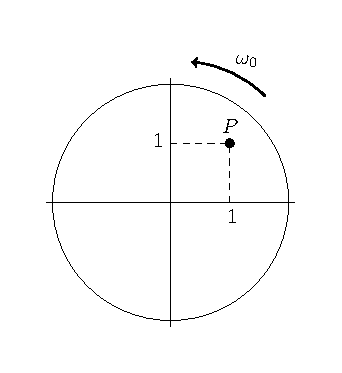
\includegraphics[scale=1]{Imagenes/Ejercicio_Disco_Rotando_01.eps}
\end{figure}
\begin{enumerate}[label=\alph*)]
\item En coordenadas cartesianas, ¿cuál es el vector velocidad del punto $P$ localizado en las coordenadas cartesianas $(1, 1)$?
\item En coordenadas polares, ¿cuál es el vector velocidad del punto $P$ localizado en las coordenadas cartesianas $(1, 1)$?
\end{enumerate}
%Ref. Kusse (2006) Chap. 3 Exercises 17
\item Considera una función escalar de la posición $\Phi$ que en coordenadas cilíndricas $(\rho, \phi, z)$ es tal que $\Phi = \rho \, \cos \phi$.
\begin{enumerate}[label=\roman*)]
\item Describe las superficies constantes $\phi$ en el plano $x-y$.
\item Sea el vector $\vb{V} = \grad{\Phi}$. Calcula las componentes radial $V_{\rho}$ y azimutal $V_{\phi}$ del vector $\vb{V}$.
\end{enumerate} 
%Ref. Kusse (2006) Chap. 3 Exercises 19
\item Considera una esfera de radio $r_{0}$, que gira a una velocidad constante $\omega_{0}$ alrededor del eje $z$, tal que:
\begin{align*}
\bm{\omega} = \omega_{0} \, \vu{e}_{z}
\end{align*}
\begin{enumerate}[label=\alph*)]
\item Determina una expresión para el vector velocidad $\vb{v}$ de puntos en la superficie de la esfera usando coordenadas esféricas y vectores base esféricos. Recuerda que $\vb{v} = \bm{\omega} \cp \vb{r}$.
\item Integra:
\begin{align*}
\scaleoint{6ex} \dd{\vb{r}} \cdot \vb{v}
\end{align*}
alrededor del ecuador de la esfera.
\item Ahora resuelva la integral de superficie:
\begin{align*}
\scaleoint{6ex} \dd{\bm{\sigma}} \cp \vb{v}
\end{align*}
sobre la superficie completa de la esfera.
\end{enumerate}

%Ref. Boas (2005) Section 8. Problems 9. pag. 525
\item Con el sistema de coordenadas bipolar $(u, v)$:
\begin{align*}
x &= \dfrac{a \, \sinh u}{\cosh u + \cos v} \\[0.5em]
y &= \dfrac{a \, \sin v}{\cosh u + \cos v}
\end{align*}
\begin{enumerate}[label=\alph*)]
\item Describe las superficies coordenadas que se generan.
\item \label{inciso_1_b} Determina el elemento $\dd{\vb{s}}$ y de los vectores unitarios $\vu{e}$, calcula las componentes de la velocidad y la aceleración.
\end{enumerate}
\item En el sistema coordenado bipolar, calcula los operadores diferenciales: gradiente, divergencia, rotacional y laplaciano.
%Ref. Boas (2005) Section 9. Problemas 3
% \item Usando coordenadas bipolares, escribe las ecuaciones de Lagrange para el movimiento de una partícula sobre la que actúa una fuerza $\vb{F} = - \grad{V}$, donde $V$ es la energía potencial. Divide cada ecuación de Lagrange por el factor de escala correspondiente para que los componentes de $\vb{F}$ (es decir, de $- \grad{V}$) aparezcan en las ecuaciones. Por tanto, escribe las ecuaciones como las ecuaciones componentes de $\vb{F} = m \, \vb{a}$, y así encuentra las componentes de la aceleración $\vb{a}$. Compara los resultados con el Problema 1 \ref{inciso_1_b}.
%Ref. Arfken (1981) 2.10.1
\item Utilizando $\xi = \cosh u$, $\eta = \cos v$, demuestra que el elemento de volumen en las coordenadas esferoidales prolatas obtenido mediante la transformación directa de la siguiente igualdad:
\begin{align*}
\dd{\tau} = a^{3} \, \big( \sinh^{2} u + \sin^{2} v \big) \, \sinh u \, \sin v \dd{u} \dd{v} \dd{\varphi}
\end{align*}
es:
\begin{align*}
\dd{\tau} = - a^{3} \, \big( \xi^{2} - \eta^{2} \big) \dd{\xi} \dd{\eta} \dd{\varphi}
\end{align*}
% %Ref Arfken (2006) 8.1.6
% \item Transformando la integral a una función Gamma, demuestra que:
% \begin{align*}
% - \scaleint{6ex}_{\bs 0}^{1} x^{k} \, \ln x \dd{x} = \dfrac{1}{(k + 1)^{2}} \hspace{1.5cm} k > -1
% \end{align*}
%Ref Arfken (2006) 8.1.13
\item Para $s$ entero no negativo, demuestra que:
\begin{align*}
(- 2 s - 1)!! = \dfrac{(-1)^{s}}{(2 s - 1)!!} = \dfrac{(-1)^{s} \, 2^{s} \, s!}{(2 s)!}
\end{align*}
%Ref Arfken (2006) 8.1.17
\item \begin{enumerate}[label=\alph*)]
\item Demuestra que:
\begin{align*}
\Gamma \bigg( \dfrac{1}{2} - n \bigg) \, \Gamma \bigg( \dfrac{1}{2} + n \bigg) = (-1)^{n} \, \pi
\end{align*}
donde $n$ es un entero.
\item Expresa $\Gamma \bigg( \dfrac{1}{2} + n \bigg)$ y $\Gamma \bigg( \dfrac{1}{2} - n \bigg)$ por separado en términos de $\pi^{\frac{1}{2}}$ y del doble factorial.
\end{enumerate}
%Ref. Arfken (2006) 8.4.6
\item Demuestra que al evaluar la siguiente integral:
\begin{align*}
I = \scaleint{6ex}_{\bs -1}^{1} (1 + x)^{a} \, (1 - x)^{b} \dd{x}
\end{align*}
en términos de la función Beta, se expresa como:
\begin{align*}
I = 2^{a+b+1} \, B \big( a + 1, b + 1 \big)
\end{align*}
\end{enumerate}
\end{document}